% Options for packages loaded elsewhere
\PassOptionsToPackage{unicode}{hyperref}
\PassOptionsToPackage{hyphens}{url}
\PassOptionsToPackage{dvipsnames,svgnames,x11names}{xcolor}
%
\documentclass[
  a4paper,
]{article}

\usepackage{amsmath,amssymb}
\usepackage{iftex}
\ifPDFTeX
  \usepackage[T1]{fontenc}
  \usepackage[utf8]{inputenc}
  \usepackage{textcomp} % provide euro and other symbols
\else % if luatex or xetex
  \usepackage{unicode-math}
  \defaultfontfeatures{Scale=MatchLowercase}
  \defaultfontfeatures[\rmfamily]{Ligatures=TeX,Scale=1}
\fi
\usepackage{lmodern}
\ifPDFTeX\else  
    % xetex/luatex font selection
\fi
% Use upquote if available, for straight quotes in verbatim environments
\IfFileExists{upquote.sty}{\usepackage{upquote}}{}
\IfFileExists{microtype.sty}{% use microtype if available
  \usepackage[]{microtype}
  \UseMicrotypeSet[protrusion]{basicmath} % disable protrusion for tt fonts
}{}
\makeatletter
\@ifundefined{KOMAClassName}{% if non-KOMA class
  \IfFileExists{parskip.sty}{%
    \usepackage{parskip}
  }{% else
    \setlength{\parindent}{0pt}
    \setlength{\parskip}{6pt plus 2pt minus 1pt}}
}{% if KOMA class
  \KOMAoptions{parskip=half}}
\makeatother
\usepackage{xcolor}
\usepackage[paperwidth=8.00in,paperheight=10.00in,left=1.25in,textwidth=
5.25in,top=1.00in,textheight=8.25in]{geometry}
\setlength{\emergencystretch}{3em} % prevent overfull lines
\setcounter{secnumdepth}{5}
% Make \paragraph and \subparagraph free-standing
\makeatletter
\ifx\paragraph\undefined\else
  \let\oldparagraph\paragraph
  \renewcommand{\paragraph}{
    \@ifstar
      \xxxParagraphStar
      \xxxParagraphNoStar
  }
  \newcommand{\xxxParagraphStar}[1]{\oldparagraph*{#1}\mbox{}}
  \newcommand{\xxxParagraphNoStar}[1]{\oldparagraph{#1}\mbox{}}
\fi
\ifx\subparagraph\undefined\else
  \let\oldsubparagraph\subparagraph
  \renewcommand{\subparagraph}{
    \@ifstar
      \xxxSubParagraphStar
      \xxxSubParagraphNoStar
  }
  \newcommand{\xxxSubParagraphStar}[1]{\oldsubparagraph*{#1}\mbox{}}
  \newcommand{\xxxSubParagraphNoStar}[1]{\oldsubparagraph{#1}\mbox{}}
\fi
\makeatother

\usepackage{color}
\usepackage{fancyvrb}
\newcommand{\VerbBar}{|}
\newcommand{\VERB}{\Verb[commandchars=\\\{\}]}
\DefineVerbatimEnvironment{Highlighting}{Verbatim}{commandchars=\\\{\}}
% Add ',fontsize=\small' for more characters per line
\usepackage{framed}
\definecolor{shadecolor}{RGB}{241,243,245}
\newenvironment{Shaded}{\begin{snugshade}}{\end{snugshade}}
\newcommand{\AlertTok}[1]{\textcolor[rgb]{0.68,0.00,0.00}{#1}}
\newcommand{\AnnotationTok}[1]{\textcolor[rgb]{0.37,0.37,0.37}{#1}}
\newcommand{\AttributeTok}[1]{\textcolor[rgb]{0.40,0.45,0.13}{#1}}
\newcommand{\BaseNTok}[1]{\textcolor[rgb]{0.68,0.00,0.00}{#1}}
\newcommand{\BuiltInTok}[1]{\textcolor[rgb]{0.00,0.23,0.31}{#1}}
\newcommand{\CharTok}[1]{\textcolor[rgb]{0.13,0.47,0.30}{#1}}
\newcommand{\CommentTok}[1]{\textcolor[rgb]{0.37,0.37,0.37}{#1}}
\newcommand{\CommentVarTok}[1]{\textcolor[rgb]{0.37,0.37,0.37}{\textit{#1}}}
\newcommand{\ConstantTok}[1]{\textcolor[rgb]{0.56,0.35,0.01}{#1}}
\newcommand{\ControlFlowTok}[1]{\textcolor[rgb]{0.00,0.23,0.31}{\textbf{#1}}}
\newcommand{\DataTypeTok}[1]{\textcolor[rgb]{0.68,0.00,0.00}{#1}}
\newcommand{\DecValTok}[1]{\textcolor[rgb]{0.68,0.00,0.00}{#1}}
\newcommand{\DocumentationTok}[1]{\textcolor[rgb]{0.37,0.37,0.37}{\textit{#1}}}
\newcommand{\ErrorTok}[1]{\textcolor[rgb]{0.68,0.00,0.00}{#1}}
\newcommand{\ExtensionTok}[1]{\textcolor[rgb]{0.00,0.23,0.31}{#1}}
\newcommand{\FloatTok}[1]{\textcolor[rgb]{0.68,0.00,0.00}{#1}}
\newcommand{\FunctionTok}[1]{\textcolor[rgb]{0.28,0.35,0.67}{#1}}
\newcommand{\ImportTok}[1]{\textcolor[rgb]{0.00,0.46,0.62}{#1}}
\newcommand{\InformationTok}[1]{\textcolor[rgb]{0.37,0.37,0.37}{#1}}
\newcommand{\KeywordTok}[1]{\textcolor[rgb]{0.00,0.23,0.31}{\textbf{#1}}}
\newcommand{\NormalTok}[1]{\textcolor[rgb]{0.00,0.23,0.31}{#1}}
\newcommand{\OperatorTok}[1]{\textcolor[rgb]{0.37,0.37,0.37}{#1}}
\newcommand{\OtherTok}[1]{\textcolor[rgb]{0.00,0.23,0.31}{#1}}
\newcommand{\PreprocessorTok}[1]{\textcolor[rgb]{0.68,0.00,0.00}{#1}}
\newcommand{\RegionMarkerTok}[1]{\textcolor[rgb]{0.00,0.23,0.31}{#1}}
\newcommand{\SpecialCharTok}[1]{\textcolor[rgb]{0.37,0.37,0.37}{#1}}
\newcommand{\SpecialStringTok}[1]{\textcolor[rgb]{0.13,0.47,0.30}{#1}}
\newcommand{\StringTok}[1]{\textcolor[rgb]{0.13,0.47,0.30}{#1}}
\newcommand{\VariableTok}[1]{\textcolor[rgb]{0.07,0.07,0.07}{#1}}
\newcommand{\VerbatimStringTok}[1]{\textcolor[rgb]{0.13,0.47,0.30}{#1}}
\newcommand{\WarningTok}[1]{\textcolor[rgb]{0.37,0.37,0.37}{\textit{#1}}}

\providecommand{\tightlist}{%
  \setlength{\itemsep}{0pt}\setlength{\parskip}{0pt}}\usepackage{longtable,booktabs,array}
\usepackage{calc} % for calculating minipage widths
% Correct order of tables after \paragraph or \subparagraph
\usepackage{etoolbox}
\makeatletter
\patchcmd\longtable{\par}{\if@noskipsec\mbox{}\fi\par}{}{}
\makeatother
% Allow footnotes in longtable head/foot
\IfFileExists{footnotehyper.sty}{\usepackage{footnotehyper}}{\usepackage{footnote}}
\makesavenoteenv{longtable}
\usepackage{graphicx}
\makeatletter
\def\maxwidth{\ifdim\Gin@nat@width>\linewidth\linewidth\else\Gin@nat@width\fi}
\def\maxheight{\ifdim\Gin@nat@height>\textheight\textheight\else\Gin@nat@height\fi}
\makeatother
% Scale images if necessary, so that they will not overflow the page
% margins by default, and it is still possible to overwrite the defaults
% using explicit options in \includegraphics[width, height, ...]{}
\setkeys{Gin}{width=\maxwidth,height=\maxheight,keepaspectratio}
% Set default figure placement to htbp
\makeatletter
\def\fps@figure{htbp}
\makeatother
% definitions for citeproc citations
\NewDocumentCommand\citeproctext{}{}
\NewDocumentCommand\citeproc{mm}{%
  \begingroup\def\citeproctext{#2}\cite{#1}\endgroup}
\makeatletter
 % allow citations to break across lines
 \let\@cite@ofmt\@firstofone
 % avoid brackets around text for \cite:
 \def\@biblabel#1{}
 \def\@cite#1#2{{#1\if@tempswa , #2\fi}}
\makeatother
\newlength{\cslhangindent}
\setlength{\cslhangindent}{1.5em}
\newlength{\csllabelwidth}
\setlength{\csllabelwidth}{3em}
\newenvironment{CSLReferences}[2] % #1 hanging-indent, #2 entry-spacing
 {\begin{list}{}{%
  \setlength{\itemindent}{0pt}
  \setlength{\leftmargin}{0pt}
  \setlength{\parsep}{0pt}
  % turn on hanging indent if param 1 is 1
  \ifodd #1
   \setlength{\leftmargin}{\cslhangindent}
   \setlength{\itemindent}{-1\cslhangindent}
  \fi
  % set entry spacing
  \setlength{\itemsep}{#2\baselineskip}}}
 {\end{list}}
\usepackage{calc}
\newcommand{\CSLBlock}[1]{\hfill\break\parbox[t]{\linewidth}{\strut\ignorespaces#1\strut}}
\newcommand{\CSLLeftMargin}[1]{\parbox[t]{\csllabelwidth}{\strut#1\strut}}
\newcommand{\CSLRightInline}[1]{\parbox[t]{\linewidth - \csllabelwidth}{\strut#1\strut}}
\newcommand{\CSLIndent}[1]{\hspace{\cslhangindent}#1}

\makeatletter
\@ifpackageloaded{bookmark}{}{\usepackage{bookmark}}
\makeatother
\makeatletter
\@ifpackageloaded{caption}{}{\usepackage{caption}}
\AtBeginDocument{%
\ifdefined\contentsname
  \renewcommand*\contentsname{Table of contents}
\else
  \newcommand\contentsname{Table of contents}
\fi
\ifdefined\listfigurename
  \renewcommand*\listfigurename{List of Figures}
\else
  \newcommand\listfigurename{List of Figures}
\fi
\ifdefined\listtablename
  \renewcommand*\listtablename{List of Tables}
\else
  \newcommand\listtablename{List of Tables}
\fi
\ifdefined\figurename
  \renewcommand*\figurename{Figure}
\else
  \newcommand\figurename{Figure}
\fi
\ifdefined\tablename
  \renewcommand*\tablename{Table}
\else
  \newcommand\tablename{Table}
\fi
}
\@ifpackageloaded{float}{}{\usepackage{float}}
\floatstyle{ruled}
\@ifundefined{c@chapter}{\newfloat{codelisting}{h}{lop}}{\newfloat{codelisting}{h}{lop}[chapter]}
\floatname{codelisting}{Listing}
\newcommand*\listoflistings{\listof{codelisting}{List of Listings}}
\makeatother
\makeatletter
\makeatother
\makeatletter
\@ifpackageloaded{caption}{}{\usepackage{caption}}
\@ifpackageloaded{subcaption}{}{\usepackage{subcaption}}
\makeatother
\ifLuaTeX
  \usepackage{selnolig}  % disable illegal ligatures
\fi
\usepackage{bookmark}

\IfFileExists{xurl.sty}{\usepackage{xurl}}{} % add URL line breaks if available
\urlstyle{same} % disable monospaced font for URLs
\hypersetup{
  pdftitle={Your title},
  pdfauthor={Your name},
  colorlinks=true,
  linkcolor={blue},
  filecolor={Maroon},
  citecolor={Blue},
  urlcolor={Blue},
  pdfcreator={LaTeX via pandoc}}

\title{Your title}
\usepackage{etoolbox}
\makeatletter
\providecommand{\subtitle}[1]{% add subtitle to \maketitle
  \apptocmd{\@title}{\par {\large #1 \par}}{}{}
}
\makeatother
\subtitle{Your subtitle}
\author{Your name}
\date{June 25, 2024}

\begin{document}
\maketitle

\bookmarksetup{startatroot}

\section*{Abstract}\label{abstract}

\markboth{Abstract}{Abstract}

This is a Quarto book template for scientific article.

To learn more about Quarto books visit
\url{https://quarto.org/docs/books}.

\textbf{Key-words:}

\textbf{How cite this template:}

\bookmarksetup{startatroot}

\section{Introduction}\label{introduction}

De acordo com Munafò et al. (2017), a pesquisa científica atual enfrenta
vários desafios. Problemas como o pequeno tamanho da amostra, pequenos
tamanhos de efeito, p-hacking e HARKing (viés positivo de publicação),
conflitos de interesse e a competição entre cientistas que trabalham
isoladamente sem combinar seus esforços, têm sido apontados como
catalizadores do que se convencionou chamar de ``crise de
reprodutibilidade'' na ciência (Baker 2016; Munafò et al. 2017).

Pesquisas apontam que mais de 70\% de pesquisadores que tentaram,
falharam em reproduzir os experimentos de outros cientistas, e mais da
metade falhou em reproduzir seus próprios experimentos (Baker, 2016),
com estimativa de que 85\% dos esforços de pesquisas estejam sendo
desperdiçados (Munafò et al. 2017), gerando custos econômicos
bilionários (Freedman, Cockburn, and Simcoe 2015). A despeito daqueles
que advogam que não existe essa tal ``crise de reprodutibilidade''
(Bernard 2023; Fanelli 2018; Protzko et al. 2023), a grande maioria da
comunidade científica concorda com sua existência e defende a melhoria
da transparência, reprodutibilidade e eficiência na ciência (Baker,
2016).

Nesse contexto, o movimento da Ciência Aberta (CA) tem ganhado
notoriedade e mudado a percepção sobre o cenário científico global
(Crüwell et al. 2019). Ele busca tornar o conhecimento científico mais
acessível, transparente e colaborativo. Se apresenta como uma coleção de
práticas de democratização do conhecimento e ruptura com o formato único
de divulgação do conhecimento científico (Crüwell et al. 2019; Heinz and
Miranda 2024; Munafò et al. 2017). Ele surge do embate entre aqueles que
buscam compartilhar o conhecimento e aqueles que defendem mecanismos de
apropriação privada para a produção científica (Heinz and Miranda 2024).

A CA é um termo múltiplo e genérico (Vicente-Saez and Martinez-Fuentes
2018), que representa diversas interpretações, e é considerada um novo
modelo de divulgação e produção de resultados científicos por meio do
acesso livre e irrestrito ao conhecimento (Heinz and Miranda 2024). A CA
não é apenas um conceito, mas uma prática multifacetada que influencia o
ciclo de vida da pesquisa, desde a concepção até a disseminação dos
resultados (Silva and Silveira 2019). Existem pelo menos cinco escolas
de pensamento dentro da CA. Estas escolas abrangem desde a arquitetura
tecnológica necessária para suportar a ciência até a inclusão do público
geral na criação de conhecimento, passando pela medição do impacto
alternativo, acesso ao conhecimento como um direito humano, e a pesquisa
colaborativa como inovação aberta (Silva and Silveira 2019). A taxonomia
proposta pela FOSTER (Facilitate Open Science Training for Eurpean
Research)(https://www.fosteropenscience.eu/foster-taxonomy/open-workflow-tools),
e sua releitura revisada e ampliada para o contexto latino americano por
Silveira et al.~(2023), tendo em vista as recomendações da UNESCO
(2021), nos dá uma dimensão da complexidade do assunto (vide ilustração
em: https://doi.org/10.5281/zenodo.7836884). Existem vários argumentos
que sustentam a importância da CA (Heinz and Miranda 2024).
Primeiramente, a CA pode trazer benefícios sociais significativos, pois
contribui para o avanço do conhecimento, a inovação, a educação, a
transparência e a participação cidadã. Além disso, a CA pode trazer
benefícios científicos ao aumentar a qualidade, a reprodutibilidade, a
eficiência e o impacto da pesquisa científica. Ela também facilita a
colaboração, a comunicação e a interdisciplinaridade entre os
pesquisadores. Por fim, a CA pode trazer benefícios éticos ao promover a
integridade, a responsabilidade, a equidade e a diversidade na ciência,
além de respeitar os direitos dos autores, dos participantes e da
sociedade como um todo. Esses argumentos são fundamentais para legitimar
a CA e destacar sua importância no mundo atual (Heinz and Miranda 2024),
principalmente, como potencial transformador para reduzir desigualdades
existentes em tecnologias de informação e comunicação -- reduzir
exclusões digitais, tecnológicas e de conhecimento --, e acelerar o
progresso rumo à implementação da Agenda 2030 e realização dos Objetivos
de Desenvolvimento Sustentável (UNESCO 2021). O movimento da CA no
Brasil está em uma fase transitória (Rezende and Falgueras 2020) --
ainda consolidando o acesso aberto -- com o governo desempenhando um
papel crucial nesse processo. O Brasil tem ganhado destaque por sua
abordagem única na implementação da CA. Esta abordagem é moldada por
marcos regulatórios que se estendem desde o governo até as instituições
e agências de financiamento. Os regulamentos brasileiros,
particularmente aqueles que promovem a abertura de dados governamentais,
têm um impacto direto na prática científica. Eles incentivam a
transparência e facilitam o acesso a dados científicos originados de
instituições públicas (Rezende and Falgueras 2020). A trajetória
brasileira rumo à CA inicia com a abertura de dados na esfera
governamental entre 2009 e 2016, evoluindo para a criação de um grupo de
trabalho em 2017 pelo Ministério da Ciência, Tecnologia, Inovações e
Comunicações (MCTIC) para desenvolver uma política nacional para a CA.
Este esforço concentrou ênfase no reconhecimento dos dados de pesquisa
como ativos de desenvolvimento científico, econômico e social, buscando
facilitar seu acesso, compartilhamento e reutilização (Rezende and
Falgueras 2020). Talvez por esse motivo, as políticas institucionais
brasileiras revelam um cenário ainda muito influenciado pela ``via
verde'' do movimento de acesso aberto, caracterizado pelo depósito de
dados em repositórios digitais abertos, e que o comprometimento efetivo
do Brasil com a CA ainda é incipiente. As regulamentações atuais
favorecem principalmente o acesso aberto, sem abordar de maneira
abrangente outros aspectos da CA (Rezende and Falgueras 2020). O Brasil
é um dos líderes mundiais no fornecimento de acesso universal às suas
pesquisas e estudos (Neto, Willinsky, and Alperin 2016), com crescimento
estável de sua produção científica disponível em acesso aberto,
principalmente, as áreas de Agricultura e Ciência \& Tecnologia
(Caballero-Rivero, Sánchez-Tarragó, and dos Santos 2019). Em termos de
pesquisa acadêmica sobre o tema no Brasil, os estudos são precoces e
concentrados na área de Ciência da Informação (Albano, Pedroso, and
Caetano 2023). A despeito da maturidade da CA no Brasil, a importância
do tema -- materializada na quantidade de produção acadêmica -- tem
aumentado vertiginosamente (Albano, Pedroso, and Caetano 2023), e a
dispersão de autores e respectivas instituições que publicam sobre o
assunto, parece ser a situação predominante. Apesar de importantes
atores nacionais, tais como CAPES, CNPq e Scielo, defenderem o
crescimento de iniciativas de CA (Mendes-Da-Silva 2023), o assunto no
Brasil parece estar circunscrito em iniciativas de importantes
periódicos nacionais sobre dados aberto, capitaneados pelas orientações
da Scielo. Não foi encontrada nenhuma pesquisa empírica, sobre a prática
da CA no Brasil. Por prática de CA entende-se a perspectiva micro da CA,
relacionadas com as terminologias e conhecimento em torno do fluxo de
trabalho do gerador de conhecimento científico aberto (vide ilustração
em: https://doi.org/10.5281/zenodo.10835001), ou seja, o cientista em
gestão que se propõe tornar sua pesquisa transparente, reprodutível e
replicável. Exclui-se a perspectiva macro, relacionadas com as
ramificações conceituais da CA concernentes às políticas públicas,
infraestrutura, envolvimento aberto de atores sociais e diálogo aberto
com outros sistemas de conhecimento (vide ilustração em:
https://doi.org/10.5281/zenodo.10835001). Essa última perspectiva está
fora do escopo do projeto, que se concentra em algumas das dimensões da
perspectiva micro, particularmente, as ferramentas disponíveis para
compilação dos produtos científicos que integram a publicação científica
(UNESCO 2021). Apesar de uma verossímil expectativa desabonadora, tendo
em vista a contexto da CA no Brasil, o diagnóstico da situação da
prática da CA se mostra importante, per si, pois: 1) ajuda a compreender
a natureza exata do problema, suas causas, efeitos e riscos; 2) auxilia
a alocação eficiente de recursos pelos atores envolvidos (e.g., os
programas de pós-graduação podem direcionar os recursos para onde eles
são mais necessários e onde terão o maior impacto; 3) orienta
indicadores de desempenho e metas realistas, o que facilita a avaliação
do progresso e a eficácia das ações tomadas; 4) permite que os atores
envolvidos aprendam com os problemas enfrentados, adaptando-se e
melhorando suas estratégias e processos para o futuro; e 5) torna
possível desenvolver soluções ou intervenções que sejam diretamente
direcionadas ao problema em questão, aumentando as chances de sucesso.
Sobre esse último ponto, até para aqueles que não reconhecem a ``crise
de reprodutibilidade'' na ciência (Bernard 2023), a comunidade
científica e atores importantes do cenário advogam que a solução inclui
educar os estudantes e pesquisadores desde cedo em todas as questões da
CA (Baker et al., 2023; Bezjak et al., 2018; Chopik et al., 2018;
Crüwell et al., 2019; Dogucu \& Çetinkaya-Rundel, 2022; Janz, 2015;
McAleer et al., 2022; Munafò et al., 2017; Toelch \& Ostwald, 2018). A
referida crise não deriva de má conduta científica, mas principalmente
da confusão entre replicar conclusões, replicar resultados, falta de
educação em estatística, lógica científica, método científico,
alfabetização de dados, etc. Para combater essas questões é necessário
investir em educação e disseminação de boas práticas de investigação
para uma mudança de cultura (Baker et al., 2023; Bezjak et al., 2018;
Chopik et al., 2018; Crüwell et al., 2019; Dogucu \& Çetinkaya-Rundel,
2022; Heinz \& Miranda, 2024; Janz, 2015; McAleer et al., 2022; Munafò
et al., 2017; Toelch \& Ostwald, 2018).

Investir em recursos humanos, treinamento, educação, alfabetização
digital, capacitação sistemática e contínua, e fomentar uma cultura
científica de CA, têm sido apresentadas como algumas das principais
medidas simultâneas para superar o cenário atual (Committee on
Reproducibility and Replicability in Science et al. 2019; European
Commission. Directorate General for Research and Innovation. 2017;
UNESCO 2021).\\
A proposta do presente projeto de pesquisa pode contribuir para a
literatura da CA no Brasil, pois pretende perseguir dois objetivos
concomitantes: 1) diagnosticar sua prática junto aos pesquisadores
brasileiros; e 2) promover o desenvolvimento de uma intervenção
educacional sobre a prática (workflow) e principais ferramentas para
compilação dos produtos científicos que integram uma publicação
científica aberta. Sobre o primeiro objetivo, os detalhes serão
apresentados num pré-registro (\textbf{vantveer2016?}) que
disponibilizaremos após a aprovação do projeto, seguindo as boas
práticas de CA (Gilroy and Kaplan 2019; \textbf{kathawalla2021?};
\textbf{klein2018?}), no entanto, em termos de delineamento pode-se
adiantar que a partir da população-alvo, faremos a tradução e adaptação
transcultural (\textbf{behr2016?}) do instrumento de medida de Ferguson
et al.~(2023), que pelas nossas pesquisas preliminares, se mostrou a
pesquisa mais ampla e confiável sobre atitudes, usabilidade e percepção
sobre as práticas de CA junto a pesquisadores. Em português não existe
nenhum instrumento de medida válido e confiável sobre esses construtos,
e esse objetivo per si, pode ser considerado um produto científico. Em
posse do instrumento de medida válido e confiável, seguindo as melhores
práticas da literatura psicométrica (\textbf{bandalos2018?};
\textbf{cohen2022?}; \textbf{furr2021?}; \textbf{rogers2024?};
\textbf{rogers2022?}; \textbf{urbina2014?}) e diretrizes da pesquisa
original (\textbf{ferguson2023?}) para sua replicação, em outra amostra
da população-alvo, diagnosticaremos o panorama geral da prática de CA no
Brasil. Essa segunda amostra será coletada em dois momentos: i) antes da
intervenção (pré-teste) e ii) depois da intervenção (pós-teste).
Coletaremos informações de indivíduos que realizarão (grupo
experimental) e não realização (grupo controle) o treinamento em
práticas de CA (tratamento/intervenção). Os participantes serão
convidados aleatoriamente -- via e-mail e comunicação durante a
intervenção para preenchimento de um questionário on-line -- para cada
um dos grupos. Não teremos a pretensão de escapar do viés de autoseleção
e abandono, devido a característica do delineamento. A amostra que
buscará estabelecer uma linha de base (pré-teste) para o treinamento,
pode ser utilizada para reflexões sobre o panorama geral da prática de
CA no Brasil. No entanto, com a implementação da intervenção e posterior
aplicação do pós-teste, poderemos comparar os resultados dentro de cada
grupo e medida repetida para avaliar a eficácia do treinamento no
quase-experimento. Utilizaremos as técnicas estatísticas adequadas para
a design metodológico da pesquisa, circunscritas no arcabouço da
Modelagem de Equações Estruturais (\textbf{hair2019book?};
\textbf{hoyle2023?}; \textbf{kline2023?}), e seguiremos de perto algumas
propostas de workflow para a reprodutibilidade, replicabilidade e
transparência da pesquisas (\textbf{mang2023?}; \textbf{peikert2021?};
\textbf{peikert2021a?}; \textbf{vanlissa2021?}), conforme preconizadas
nas boas práticas de CA (Gilroy and Kaplan 2019;
\textbf{kathawalla2021?}; \textbf{klein2018?}). Diferente do primeiro
objetivo, que no presente projeto foi apenas esboçado, o segundo
objetivo, quando do começo do projeto, espera-se que esteja com escopo
concluído nos moldes recomendados pela literatura de CA (Dogucu and
Çetinkaya-Rundel 2022). Isso porque o conteúdo do curso faz parte do dia
a dia dos proponentes desse projeto. As ferramentas que serão
ministradas no curso (OSF, Zotero, Git/Github, Zenodo, RStudio, Quarto,
Docker, etc.) fazem parte do workflow de trabalho dos proponentes, e o
curso, está sendo concebido enquanto projeto de extensão universitária
(https://phdpablo.github.io/curso-open-science/), e será ministrado pelo
menos uma vez como piloto no ano corrente. Cremos que adiantar esse
piloto nos ajudará i) avaliar se a intervenção pode ser implementada
como planejado no contexto real; ii) identificar e corrigir quaisquer
problemas ou falhas na concepção da intervenção antes de realizar o
estudo; iii) ajustar os materiais, recursos, métodos e procedimentos
operacionais do treinamento para melhorar a eficácia e a eficiência; iv)
familiarizar com o processo e resolver quaisquer dificuldades
operacionais; v) garantir que todos os envolvidos compreendam e sigam o
protocolo de pesquisa corretamente (\textbf{janghorban2014?}), reduzindo
a variabilidade na implementação; v) identificar potenciais problemas
éticos; e vi) definir expectativas realistas sobre os resultados e o
impacto da intervenção, tanto para os pesquisadores quanto para os
participantes (\textbf{kezar2000?}; \textbf{thabane2010?}). Esse
quase-experimento como uma pesquisa-ação, em um contexto universitário,
integra de forma profícua as atividades de ensino, pesquisa e extensão
universitária (\textbf{estevescampos2020?}), promovendo a
indissociabilidade, interdisciplinaridade, multidimensionalidade,
integração e articulação dessa tríade, quase sempre inexistente em
grande parte dos projetos de pesquisa nas universidade brasileiras
(\textbf{farias2010?}), porém de suma importância
(\textbf{goncalves2015?}). Nesse sentido, esse projeto de pesquisa se
associa à um projeto de ensino por proporcionar uma experiência de
aprendizagem integrada para os envolvidos na academia, desenvolvendo
habilidades e competências essenciais (\textbf{moita2009?}). Como
projeto de extensão, ele transcende os limites da universidade,
aplicando o conhecimento gerado para beneficiar a comunidade mais ampla
e promover mudanças sociais positivas (\textbf{rays2012?}),
principalmente, através da comunicação científica
(\textbf{targino2000?}).

\bookmarksetup{startatroot}

\section{Background}\label{background}

In summary, this article has no content whatsoever.

\begin{Shaded}
\begin{Highlighting}[]
\DecValTok{1} \SpecialCharTok{+} \DecValTok{1}
\end{Highlighting}
\end{Shaded}

\begin{verbatim}
[1] 2
\end{verbatim}

\bookmarksetup{startatroot}

\section{Methods}\label{methods}

\bookmarksetup{startatroot}

\section{Results}\label{results}

This a Quarto document. To learn more about Quarto see
\url{https://quarto.org}.

Click the \textbf{Code} button in the header to see the full source code
of this document.

Here we call the R \texttt{summary()} function---the function's output
is included immediately below:

\begin{Shaded}
\begin{Highlighting}[]
\FunctionTok{summary}\NormalTok{(cars)}
\end{Highlighting}
\end{Shaded}

\begin{verbatim}
     speed           dist       
 Min.   : 4.0   Min.   :  2.00  
 1st Qu.:12.0   1st Qu.: 26.00  
 Median :15.0   Median : 36.00  
 Mean   :15.4   Mean   : 42.98  
 3rd Qu.:19.0   3rd Qu.: 56.00  
 Max.   :25.0   Max.   :120.00  
\end{verbatim}

\subsection{Plot Output}\label{plot-output}

You can also embed plots, for example:

\begin{Shaded}
\begin{Highlighting}[]
\FunctionTok{library}\NormalTok{(ggplot2)}
\NormalTok{dat }\OtherTok{\textless{}{-}} \FunctionTok{data.frame}\NormalTok{(}\AttributeTok{cond =} \FunctionTok{rep}\NormalTok{(}\FunctionTok{c}\NormalTok{(}\StringTok{"A"}\NormalTok{, }\StringTok{"B"}\NormalTok{), }\AttributeTok{each=}\DecValTok{10}\NormalTok{),}
                  \AttributeTok{xvar =} \DecValTok{1}\SpecialCharTok{:}\DecValTok{20} \SpecialCharTok{+} \FunctionTok{rnorm}\NormalTok{(}\DecValTok{20}\NormalTok{,}\AttributeTok{sd=}\DecValTok{3}\NormalTok{),}
                  \AttributeTok{yvar =} \DecValTok{1}\SpecialCharTok{:}\DecValTok{20} \SpecialCharTok{+} \FunctionTok{rnorm}\NormalTok{(}\DecValTok{20}\NormalTok{,}\AttributeTok{sd=}\DecValTok{3}\NormalTok{))}

\FunctionTok{ggplot}\NormalTok{(dat, }\FunctionTok{aes}\NormalTok{(}\AttributeTok{x=}\NormalTok{xvar, }\AttributeTok{y=}\NormalTok{yvar)) }\SpecialCharTok{+}
    \FunctionTok{geom\_point}\NormalTok{(}\AttributeTok{shape=}\DecValTok{1}\NormalTok{) }\SpecialCharTok{+} 
    \FunctionTok{geom\_smooth}\NormalTok{() }
\end{Highlighting}
\end{Shaded}

\begin{figure}[H]

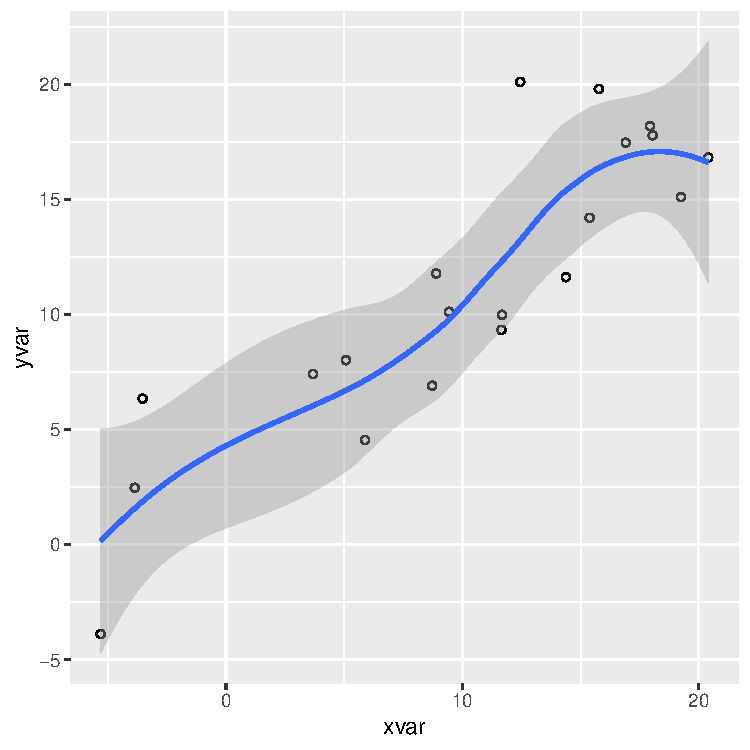
\includegraphics{04-results_files/figure-pdf/fig-pressure-1.pdf}

\caption{\label{fig-pressure}Pressure}

\end{figure}%

Note that the \texttt{code-fold:\ true} parameter was added to the code
chunk to hide the code by default (click ``Code'' above the plot to see
the code).

The use of the \texttt{label} and \texttt{fig-cap} options make this a
cross-referenceable figure (see Figure~\ref{fig-pressure}).

\subsection{Tables}\label{tables}

Use the \texttt{knitr::kable()} function to print tables as HTML:

\begin{Shaded}
\begin{Highlighting}[]
\NormalTok{knitr}\SpecialCharTok{::}\FunctionTok{kable}\NormalTok{(}\FunctionTok{head}\NormalTok{(ggplot2}\SpecialCharTok{::}\NormalTok{diamonds))}
\end{Highlighting}
\end{Shaded}

\begin{longtable}[]{@{}
  >{\raggedleft\arraybackslash}p{(\columnwidth - 18\tabcolsep) * \real{0.0952}}
  >{\raggedright\arraybackslash}p{(\columnwidth - 18\tabcolsep) * \real{0.1587}}
  >{\raggedright\arraybackslash}p{(\columnwidth - 18\tabcolsep) * \real{0.0952}}
  >{\raggedright\arraybackslash}p{(\columnwidth - 18\tabcolsep) * \real{0.1270}}
  >{\raggedleft\arraybackslash}p{(\columnwidth - 18\tabcolsep) * \real{0.0952}}
  >{\raggedleft\arraybackslash}p{(\columnwidth - 18\tabcolsep) * \real{0.0952}}
  >{\raggedleft\arraybackslash}p{(\columnwidth - 18\tabcolsep) * \real{0.0952}}
  >{\raggedleft\arraybackslash}p{(\columnwidth - 18\tabcolsep) * \real{0.0794}}
  >{\raggedleft\arraybackslash}p{(\columnwidth - 18\tabcolsep) * \real{0.0794}}
  >{\raggedleft\arraybackslash}p{(\columnwidth - 18\tabcolsep) * \real{0.0794}}@{}}
\toprule\noalign{}
\begin{minipage}[b]{\linewidth}\raggedleft
carat
\end{minipage} & \begin{minipage}[b]{\linewidth}\raggedright
cut
\end{minipage} & \begin{minipage}[b]{\linewidth}\raggedright
color
\end{minipage} & \begin{minipage}[b]{\linewidth}\raggedright
clarity
\end{minipage} & \begin{minipage}[b]{\linewidth}\raggedleft
depth
\end{minipage} & \begin{minipage}[b]{\linewidth}\raggedleft
table
\end{minipage} & \begin{minipage}[b]{\linewidth}\raggedleft
price
\end{minipage} & \begin{minipage}[b]{\linewidth}\raggedleft
x
\end{minipage} & \begin{minipage}[b]{\linewidth}\raggedleft
y
\end{minipage} & \begin{minipage}[b]{\linewidth}\raggedleft
z
\end{minipage} \\
\midrule\noalign{}
\endhead
\bottomrule\noalign{}
\endlastfoot
0.23 & Ideal & E & SI2 & 61.5 & 55 & 326 & 3.95 & 3.98 & 2.43 \\
0.21 & Premium & E & SI1 & 59.8 & 61 & 326 & 3.89 & 3.84 & 2.31 \\
0.23 & Good & E & VS1 & 56.9 & 65 & 327 & 4.05 & 4.07 & 2.31 \\
0.29 & Premium & I & VS2 & 62.4 & 58 & 334 & 4.20 & 4.23 & 2.63 \\
0.31 & Good & J & SI2 & 63.3 & 58 & 335 & 4.34 & 4.35 & 2.75 \\
0.24 & Very Good & J & VVS2 & 62.8 & 57 & 336 & 3.94 & 3.96 & 2.48 \\
\end{longtable}

\subsection{LaTeX Math}\label{latex-math}

You can also include LaTeX math:

\[
P\left(A=2\middle|\frac{A^2}{B}>4\right)
\]

\bookmarksetup{startatroot}

\section{Final Considerations}\label{final-considerations}

\bookmarksetup{startatroot}

\section*{References}\label{references}
\addcontentsline{toc}{section}{References}

\markboth{References}{References}

\phantomsection\label{refs}
\begin{CSLReferences}{1}{0}
\bibitem[\citeproctext]{ref-albano2023}
Albano, Cláudio Sonáglio, Paula de Oliveira Pedroso, and Doriedson
Oliveira Caetano. 2023. {``Ci{ê}ncia {Aberta}: {Um Panorama Sobre} as
{Publica{ç}{õ}es No Cen{á}rio Brasileiro}.''} \emph{Saber Cient{í}fico}
12 (1): 1--12.

\bibitem[\citeproctext]{ref-baker2016}
Baker, Monya. 2016. {``1,500 {Scientists Lift} the {Lid} on
{Reproducibility}.''} \emph{Nature} 533 (7604): 452--54.
\url{https://doi.org/10.1038/533452a}.

\bibitem[\citeproctext]{ref-bernard2023}
Bernard, Christophe. 2023. {``Stop {Reproducing} the {Reproducibility
Crisis}.''} \emph{Eneuro} 10 (2): ENEURO.0032--23.2023.
\url{https://doi.org/10.1523/ENEURO.0032-23.2023}.

\bibitem[\citeproctext]{ref-caballero-rivero2019}
Caballero-Rivero, Alejandro, Nancy Sánchez-Tarragó, and Raimundo Nonato
Macedo dos Santos. 2019. {``Pr{á}ticas de {Ci{ê}ncia Aberta} Da
Comunidade Acad{ê}mica Brasileira: Estudo a Partir Da Produ{ç}{ã}o
Cient{í}fica.''} \emph{Transinforma{ç}{ã}o} 31 (November): e190029.
\url{https://doi.org/10.1590/2318-0889201931e190029}.

\bibitem[\citeproctext]{ref-crrs2019}
Committee on Reproducibility and Replicability in Science, Board on
Behavioral, Cognitive, and Sensory Sciences, Committee on National
Statistics, Division of Behavioral and Social Sciences and Education,
Nuclear and Radiation Studies Board, Division on Earth and Life Studies,
Board on Mathematical Sciences and Analytics, et al. 2019.
\emph{Reproducibility and {Replicability} in {Science}}. Washington,
D.C.: National Academies Press. \url{https://doi.org/10.17226/25303}.

\bibitem[\citeproctext]{ref-cruwell2019}
Crüwell, Sophia, Johnny Van Doorn, Alexander Etz, Matthew C. Makel,
Hannah Moshontz, Jesse C. Niebaum, Amy Orben, Sam Parsons, and Michael
Schulte-Mecklenbeck. 2019. {``Seven {Easy Steps} to {Open Science}: {An
Annotated Reading List}.''} \emph{Zeitschrift f{ü}r Psychologie} 227
(4): 237--48. \url{https://doi.org/10.1027/2151-2604/a000387}.

\bibitem[\citeproctext]{ref-dogucu2022}
Dogucu, Mine, and Mine Çetinkaya-Rundel. 2022. {``Tools and
{Recommendations} for {Reproducible Teaching}.''} \emph{Journal of
Statistics and Data Science Education} 30 (3): 251--60.
\url{https://doi.org/10.1080/26939169.2022.2138645}.

\bibitem[\citeproctext]{ref-eu2017}
European Commission. Directorate General for Research and Innovation.
2017. \emph{Providing {Researchers} with the {Skills} and {Competencies
They Need} to {Practise Open Science}.} LU: Publications Office.

\bibitem[\citeproctext]{ref-fanelli2018}
Fanelli, Daniele. 2018. {``Is {Science Really Facing} a {Reproducibility
Crisis}, and {Do We Need It To}?''} \emph{Proceedings of the National
Academy of Sciences} 115 (11): 2628--31.
\url{https://doi.org/10.1073/pnas.1708272114}.

\bibitem[\citeproctext]{ref-freedman2015}
Freedman, Leonard P., Iain M. Cockburn, and Timothy S. Simcoe. 2015.
{``The {Economics} of {Reproducibility} in {Preclinical Research}.''}
\emph{PLOS Biology} 13 (6): e1002165.
\url{https://doi.org/10.1371/journal.pbio.1002165}.

\bibitem[\citeproctext]{ref-gilroy2019}
Gilroy, Shawn P., and Brent A. Kaplan. 2019. {``Furthering {Open
Science} in {Behavior Analysis}: {An Introduction} and {Tutorial} for
{Using GitHub} in {Research}.''} \emph{Perspectives on Behavior Science}
42 (3): 565--81. \url{https://doi.org/10.1007/s40614-019-00202-5}.

\bibitem[\citeproctext]{ref-heinz2024}
Heinz, Michele, and Miranda Miranda. 2024. {``Ci{ê}ncia {Aberta}:
{Argumentos} e {Desafios Para Sua Legitima{ç}{ã}o Cient{í}fica}.''}
\emph{Em Quest{ã}o} 30.
\url{https://doi.org/10.1590/1808-5245.30.135618}.

\bibitem[\citeproctext]{ref-mendes-da-silva2023}
Mendes-Da-Silva, Wesley. 2023. {``What {Lectures} and {Research} in
{Business Management Need} to {Know About Open Science}.''}
\emph{Revista de Administra{ç}{ã}o de Empresas} 63 (4): e0000--0033.
\url{https://doi.org/10.1590/s0034-759020230408x}.

\bibitem[\citeproctext]{ref-munafo2017}
Munafò, Marcus R., Brian A. Nosek, Dorothy V. M. Bishop, Katherine S.
Button, Christopher D. Chambers, Nathalie Percie Du Sert, Uri Simonsohn,
Eric-Jan Wagenmakers, Jennifer J. Ware, and John P. A. Ioannidis. 2017.
{``A {Manifesto} for {Reproducible Science}.''} \emph{Nature Human
Behaviour} 1 (1): 0021. \url{https://doi.org/10.1038/s41562-016-0021}.

\bibitem[\citeproctext]{ref-neto2016}
Neto, Silvio Carvalho, John Willinsky, and Juan Pablo Alperin. 2016.
{``Measuring, {Rating}, {Supporting}, and {Strengthening Open Access
Scholarly Publishing} in {Brazil}.''} \emph{Education Policy Analysis
Archives} 24 (May): 54--54. \url{https://doi.org/10.14507/epaa.24.2391}.

\bibitem[\citeproctext]{ref-protzko2023}
Protzko, John, Jon Krosnick, Leif Nelson, Brian A. Nosek, Jordan Axt,
Matt Berent, Nicholas Buttrick, et al. 2023. {``High {Replicability} of
{Newly Discovered Social-Behavioural Findings Is Achievable}.''}
\emph{Nature Human Behaviour}, November.
\url{https://doi.org/10.1038/s41562-023-01749-9}.

\bibitem[\citeproctext]{ref-rezende2020}
Rezende, Laura Vilela Rodrigues, and Ernest Abadal Falgueras. 2020.
{``Estado {Da Arte Dos Marcos Regulat{ó}rios Brasileiros Rumo} {à}
{Ci{ê}ncia Aberta}.''} \emph{Encontros Bibli: Revista Eletr{ô}nica de
Biblioteconomia e Ci{ê}ncia Da Informa{ç}{ã}o} 25 (September): 01--25.
\url{https://doi.org/10.5007/1518-2924.2020.e71370}.

\bibitem[\citeproctext]{ref-silva2019}
Silva, Fabiano Couto Corrêa Da, and Lúcia Da Silveira. 2019. {``O
{Ecossistema Da Ci{ê}ncia Aberta}.''} \emph{Transinforma{ç}{ã}o} 31:
e190001. \url{https://doi.org/10.1590/2318-0889201931e190001}.

\bibitem[\citeproctext]{ref-unesco2021}
UNESCO. 2021. {``{UNESCO Recommendation} on {Open Science}.''} UNESCO.
\url{https://doi.org/10.54677/MNMH8546}.

\bibitem[\citeproctext]{ref-vicente-saez2018}
Vicente-Saez, Ruben, and Clara Martinez-Fuentes. 2018. {``Open {Science
Now}: {A Systematic Literature Review} for an {Integrated
Definition}.''} \emph{Journal of Business Research} 88 (July): 428--36.
\url{https://doi.org/10.1016/j.jbusres.2017.12.043}.

\end{CSLReferences}



\end{document}
